\documentclass[journal]{IEEEtran}

\renewcommand\IEEEkeywordsname{Keywords}

\usepackage{graphicx}
\graphicspath{ {images/} }
\usepackage{tabularx}
\usepackage{pdfpages}
\usepackage{amsmath}

\pagenumbering{arabic}
\setcounter{page}{2}
\bibliographystyle{IEEEtran}

\begin{document}
	\markboth{COMPSYS701 - Advanced Digital Systems Design}{}
	
\begin{titlepage}
	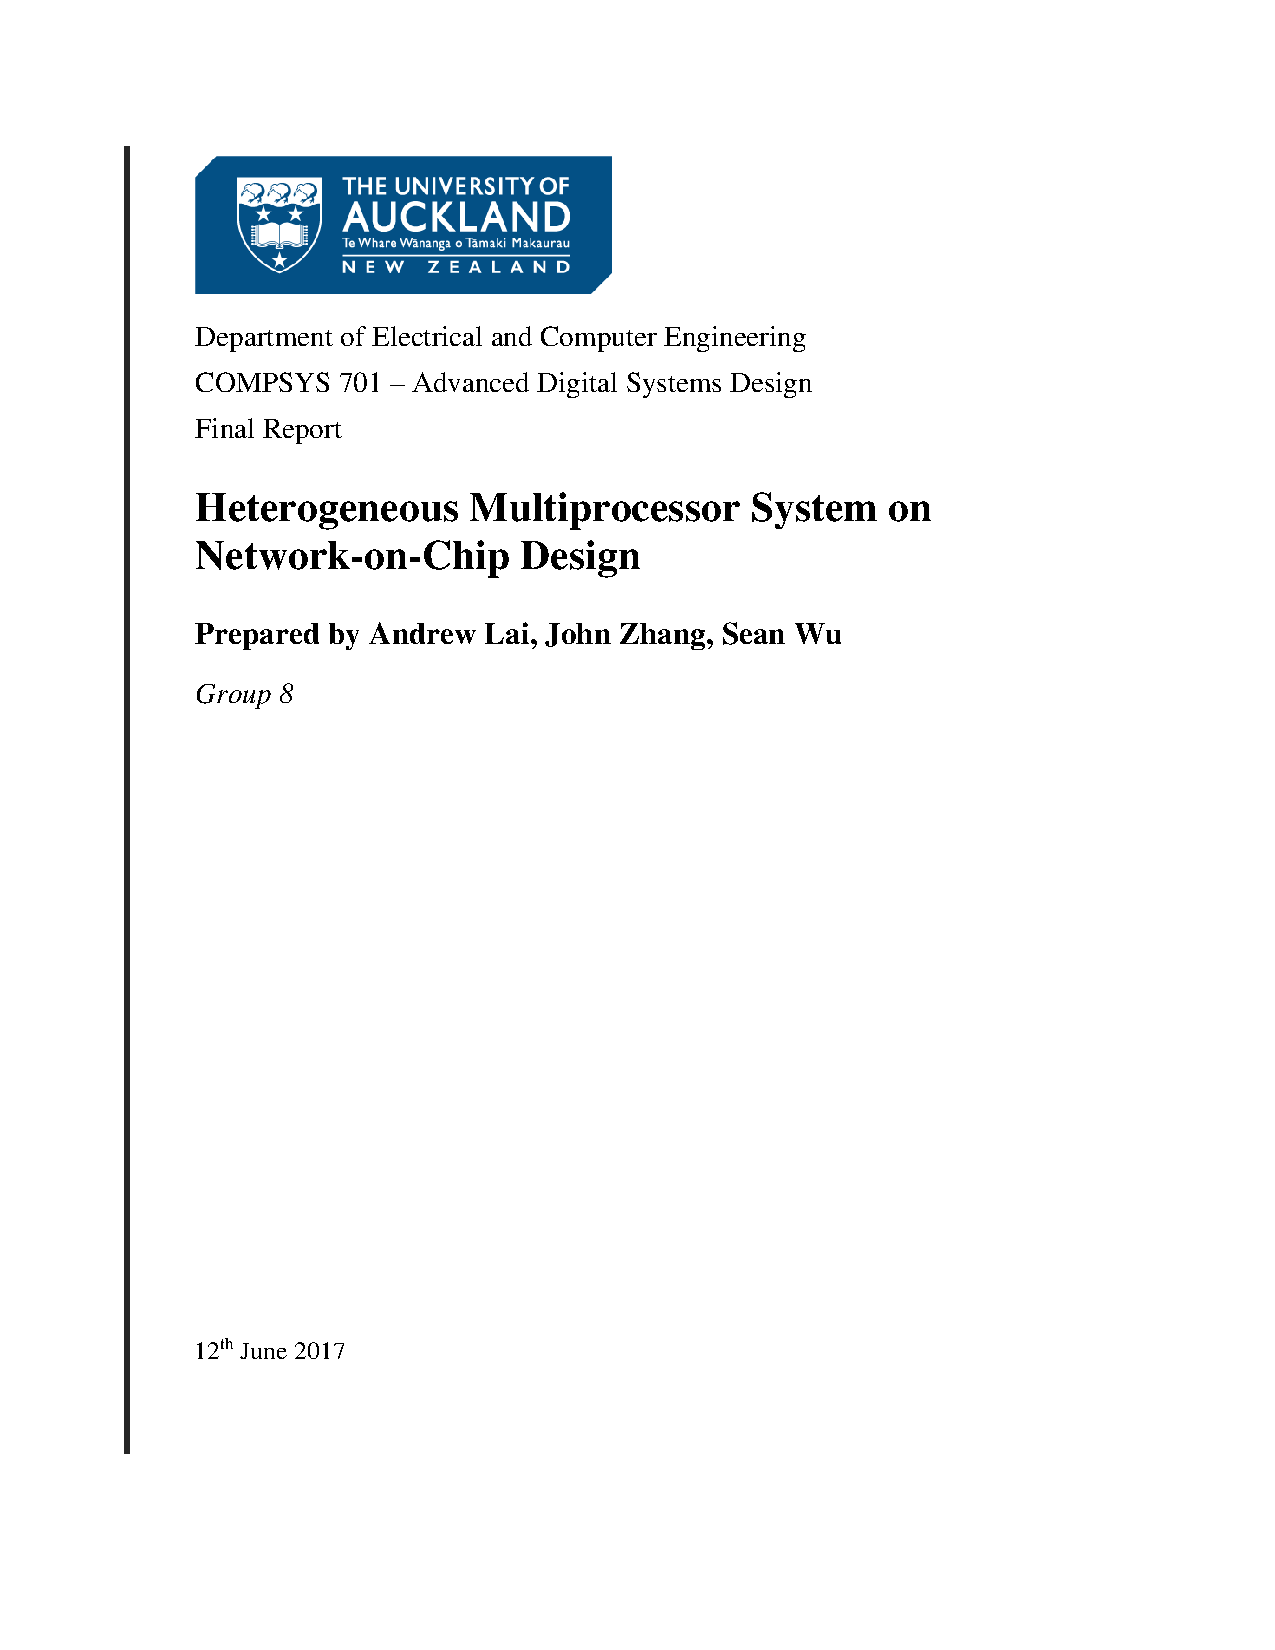
\includepdf[pages={1}]{title_page.pdf}
\end{titlepage}

	
	\title{Heterogeneous Multiprocessor System on Network-on-Chip Design}
	\author{Andrew Lai \texttt{(klai054)}, John Zhang \texttt{(szha215)}, Sean Wu \texttt{(swu145)}, group 8 - AJS \\Department of Electrical and Computer Engineering, University of Auckland, New Zealand}
	
	\maketitle
	
	\begin{abstract}
		Processors architecture size and maximum frequencies are hitting their limits. To further improve performance, multi-core systems are required.
	\end{abstract}
	
	\begin{IEEEkeywords}
		Processor design; Network-on-chip 
	\end{IEEEkeywords}
	
	
	\section{Introduction}
	Our ReCOP? mmhmmm. \\
	Our ASP/ANI? Perfection.
	
%	\begin{figure}[h!]
%		\centering
%		\includegraphics[trim={0cm, 0cm, 0cm, 0cm}, clip, width = 3.4in]{pedal_detection_fsm}
%		\caption{Pedal Detection FSM.}
%		\label{tumor_L8}
%	\end{figure}
	
	\section{Conclusion}
	Gold amongst trash.
	
	
	\section*{Appendix}
	
	
	
	
\end{document}

